\section{Normalized Systems: Impacting software stability} \label{sec_ns_theory}

\gls{ns} is a software development approach that prioritizes achieving software stability
through the use of standardized, modular components and interfaces. This theory is
informed by several scientific disciplines, including systems theory, mathematics, and
computer science, as well as some other software development approaches, such as agile
development and domain-driven design.

\gls{ns} originated in the field of software engineering. However, the underlying theory
of \gls{ns} can be applied to various other domains, such as Enterprise Engineering,
Business Process Modeling, and document management. This research acknowledges the
software engineering background of \gls{ns}. It consistently refers to software and
Information Systems when referring to \enquote*{artifacts.} However, the reader should
realize that the concepts and artifacts are not restricted to software artifacts alone.

\subsection{Towards stability} \label{subsec:on_stability}

In several disciplines, stability has been defined as \emph{Bounded Input Bounded Output}
(BIBO). It is the fundamental property of a system when subjected to bounded input
disturbances. BIBO stability ensures that the output of a system will also be bounded,
preventing uncontrolled or unexpected behavior \parencite[270]{mannaert_normalized_2016}. 

A real-world example of the importance of stability is the Tacoma Narrows Bridge in
Washington State, USA. This bridge, depicted in Figure \ref*{fig:bridge}, collapsed on
November the 7th, 1940. This was caused due to wind-induced oscillations called
aeroelastic flutter. The wind (Input) induced oscillations in the bridge, causing it to
start swaying back and forth (Output). These oscillations were initially small, but as
they continued, they began to increase in amplitude and magnitude. Eventually, this 
caused the bridge to collapse.

\begin{figure}[H]
    \centering
    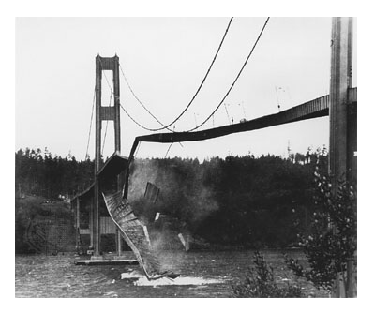
\includegraphics[width=0.6\textwidth]{Figures/bridge.pdf}
    \caption[TNB]{Tacoma Narrows Bridge (Galloping Gertie)}
    \label{fig:bridge}
\end{figure}

Stability can also be used in the context of software engineering. In the context of
\gls{ns}, it is considered a critical property that ensures that the software is not
excessively sensitive to small changes \parencite[270]{mannaert_normalized_2016}. New
functional requirements should only lead to a fixed and expected amount of changes in
the source code. 

Conversely, instabilities occur when the total number of modifications relies on the size
of the software artifact. When there are software instabilities, the number of changes
will grow over time in parallel with the growth of the system. These instabilities are
referred to as combinatorial effects \parencite[270]{mannaert_normalized_2016}. 

When combinatorial effects are absent, the software artifact can be considered evolvable.
\subsection{Towards Evolvability} \label{sec:on_evolvability}

In \gls{ns} Evolvability is a crucial property in order to achieve stable software
systems. An evolvable system can adapt over time in response to changing requirements.
\gls{ns} attempts to achieve evolvability by providing guidelines, principles and theorems
n order to achieve a modular (and scalable) architecture that allows for easy
adaptability, extensibility and the replacement of components with a minimum impact on the
quality of the functionality, and the overall structures of the architecture. This is
achieved through the use of formalized models that define the system's components,
interfaces, and behavior, as well as through the separation of concerns between different
parts of the system.

There are several aspects concerning the evolvability of software systems. One of which is
the modularity of the architecture. There is also a wide consensus about two fundamental
rules when thinking of-, and designing modularity: \emph{high cohesion} and \emph{low
coupling} \autocite[22]{mannaert_normalized_2016}.
\subsection{Modularity}

A Software module can be defined as self-contained units of code that perform specific
tasks or sets of tasks within a larger system. A software module is designed to operate
independently of other modules, with well-defined interfaces that allow it to communicate
and exchange data with other modules if necessary \autocite[22]{mannaert_normalized_2016}.

A module can be considered a hierarchical and recursive concept. They are independent of
their size (lines of code) or computational magnitude. They can be as small as a function
as part of a class. The class itself can also be considered a module. A group of classes
contained in a Dynamic Link Library (DLL) or Application Programming Interface (API) can
also be considered a module of an even bigger system. 

An important part of the design of a software system is to identify the possible different
modules and their interaction interfaces. Figure \ref{fig:modulair_components} presents a
high-level depiction of modular manifestations in the artifact, with additional examples
of modularity found in more granular implementations. Further discussion of this
architecture is provided in Chapter \ref{sec:ca_theory}.
\subsection{Cohesion} \label{subsubsec_on_cohesion}

The term cohesion denotes the extent to which the various structural components of a
software system operate cohesively towards a singular and well-defined objective or goal.
Empirical studies in software engineering have extensively demonstrated the significance
of cohesion, linking higher levels of cohesion with reduced defects, enhanced
maintainability, and greater openness to change. Consequently, achieving high cohesion has
been associated with an overall improvement in software quality attributes such as
reliability, maintainability, reusability, and evolvability.

Cohesion facilitates the reduction of complexity and interdependence among the components
of a system, thereby contributing to a more efficient, maintainable, and reliable system.
By organizing components around a shared purpose or function or by standardizing their
interfaces, data structures, and protocols, cohesion can offer the following benefits:

\begin{itemize}
    \item \textbf{Reduce redundancy and duplication of effort}: \\
    Cohesion ensures that components are arranged around a common purpose or function,
    reducing duplicates or redundant code. This simplifies system comprehension,
    maintenance, and modification.
    \item \textbf{Promoting code reuse:}\\
    Cohesion facilitates code reuse by making it easier to extract and reuse components
    designed for specific functions. This saves time and effort during development and
    enhances overall system quality.
    \item \textbf{Enhance maintainability:}\\
    Cohesion decreases the complexity and interdependence of system components, making it
    easier to identify and rectify bugs or errors in the code. This improves system
    maintainability and reduces the risk of introducing new errors during maintenance.
    \item \textbf{Increase scalability:}\\
    Cohesion improves a system's scalability by enabling it to be extended or modified
    effortlessly to accommodate changing requirements or conditions. By designing
    well-organized and well-defined components, developers can easily add or modify
    functionality as needed without disrupting the rest of the system.  
\end{itemize}


\subsection{Coupling} \label{subsec:on_coupling}

Coupling is an essential concept in software engineering that pertains to the degree of
interdependence among software modules and components. The level of coupling between
modules denotes the strength of their relationship, whereby a high level of coupling
implies a significant degree of interdependence. Conversely, low coupling signifies a
weaker relationship between modules, where modifications in one module are less likely to
impact others. Although not always possible, the level of coupling between the various
modules of the system should be kept to a bare minimum.

The negative impact of excessive coupling on software systems is considerable. High
coupling can render software systems challenging to maintain, modify, or evolve. It can make
it considerably more challenging to find the root cause of potential bugs. Additionally, it
causes fragility in the system, where slight modifications in one module can trigger
cascading failures throughout the entire system. Therefore, it is crucial for software
engineers to minimize coupling between modules while maintaining a cohesive design. By
developing systems with low coupling, software engineers can construct more maintainable,
scalable, and adaptable systems that are easier to evolve.

Coupling in software engineering can take several forms, including content, common,
control, stamp, and data coupling. Content coupling occurs when one module accesses or
modifies the internal data or logic of another module, leading to high interdependence and
difficulty in isolating errors. Common coupling occurs when several modules access and use
the same global data, increasing their interdependence and reducing modularity. Control
coupling occurs when one module controls the execution flow of another module, making it
challenging to modify or reuse the controlled module. Stamp coupling arises when two modules
share a common data structure, leading to tight coupling and high interdependence.
Finally, data coupling exists when two modules share data, which can lead to coupling
between them.

One attempt to lower coupling in the expanded artifact is to prefer stamp coupling over
data coupling through the API interface. This is done by making use of RequestModels and
ViewModels, instead of the actual data element (see example in Listings \ref{SnipModelExamples}).
Depending on the use case, only the required data is passed down to the view, or in the
case of a command accepted as an input parameter.

\lstinputlisting[
    caption={The ViewModel \parencite{koks_componentviewmodel_2023} and RequestModel
    \parencite{koks_deletecomponentcommand_2023} of the Entity 'Component'
    \parencite{koks_component_2023}},
    label={SnipModelExamples}]
    {Snippets/ModelExamples.cs}
\subsection{Expansion and code generation} \label{subsec:expansion}

Creating and maintaining a stable and evolvable system is a particularly difficult and
meticulous engineering job. Developers are required to have a sound knowledge of \gls{ns},
whilst implementing new requirements in an always consistent manner. Given the required
recurring structure, it can be perceived as a repetitive and therefore boring taks.
\parencite[219]{mannaert_normalized_2016}. On top of that, rejecting the temptation to
take shortcuts in order to follow the business's time-to-market requirements.

Given the above, it is quite logical to automate the instantiation process of software
structures and use code generation for recurring
tasks\parencite[403]{mannaert_normalized_2016}. This is where code expansion comes in
place. The concept of code expansion does not only refer to the automatic process of
adapting and maintaining software to new requirements, architectural enablers and/or
technological alterations. It also embraces manually added craftings to the software, the
so-called plugin code. These craftings are preserved after each expansion by a method that
is called harvesting and rejuvenation \parencite[405-406]{mannaert_normalized_2016}.


\subsection{The Theoretical Framework} \label{subsec:ns_desing_theorems}

\gls{ns} consists of a theoretical framework describing a set of design principles. These
principles are the basis for achieving the concepts of stability, evolvability, and
modularity. \gls{ns} provides a rigorous and mathematical foundation for these theorems
and they offer guidelines for designing and developing software systems. In the following
sections, we will focus on the principles of \gls{ns} very briefly as they have been
extensively described in various scientific papers.

We know from Chapter \ref{sec:artifact_requirements} that the design artifacts, as a part
of this research, are implemented based on the \gls{ca} principles. Therefore, contrary to
Chapter \ref{sec:ca_theory}, there will be no references to the manifestations of the NS
design theorems in the design.
\subsubsection*{Separation of Concerns}

\gls{soc} as a principle has first been mentioned by
\citeauthor{dijkstra_selected_1982}\footnote{\url{https://en.wikipedia.org/wiki/Separation_of_concerns}}
as the crucial principle to design modular software architecture
\parencite[]{dijkstra_selected_1982}. \gls{soc} promotes the idea that a program should be
divided into distinct sections, each addressing a separate concern or aspect of a design
problem. This allows for a more organized and maintainable source code. When implemented
correctly, a change to one concern does not affect the others. \gls{soc} should be applied
at the level of individual modules, rather than the level of an entire program.

\gls{soc} has been adopted as one of the design theorems of \gls{ns}, although it has a
stricter definition of this principle\parencite{mannaert_normalized_2016}.

\begin{tcolorbox}[boxrule=0.1pt, colback=mygray, title=Theorem I,colbacktitle=gray]
    \textit{A processing function can only contain a single task to achieve stability.}
\end{tcolorbox}
\subsubsection*{Data version Transparancy}

\gls{dvt} is the act of encapsulation of data entities for specific tasks at hand. This
results in the fact that data structures can have multiple versions often mentioned as
Data Transfer Objects in modern software engineering projects. In other words, it should
be possible to update the data entity without affecting the processing functions. This
leads to the following description of the theorem \parencite[280]{mannaert_normalized_2016}.

\mycolorbox{A data structure that is passed through the interface of a processing function
needs to exhibit version transparency in order to achieve stability.}{Theorem II}

\gls{dvt} is widely used in various technological applications. practically every web
service currently known supports some type of versioning. In restful APIs for example, it
is common practice to support versioning over the URI. It is considered a best practice
to encapsulate breaking changes in a new version of the endpoint/service so that the
consumers are not (directly) affected by the change. In modern Object Oriented languages,
gls{dtv} is also supported by the ability to determine the scope of visibility of the
modifiers of the various programming constructs like fields, properties, interfaces and
classes. Also known as information hiding
\parencites{parnas_criteria_1972}[278]{mannaert_normalized_2016}.
\subsubsection*{Action version Transparancy}
\gls{avt} is the property of a system to modify existing processing functions without
affecting the existing ones. It should be possible to upgrade a function without affecting
the callers of those functions. This description leads to the following theorem
\parencite[282]{mannaert_normalized_2016}.

\begin{tcolorbox}[boxrule=0.1pt, colback=mygray, title=Theorem III,colbacktitle=gray]
    \textit{A processing function that is called by another processing function, needs to exhibit version transparency in order to achieve stability.}
\end{tcolorbox}

Most of the modern technology environments support some form of \gls{avt}. Polymorphism is
a widely used technique in order to support this theorem. Specifically, parametric
polymorphism \footnote{\url{https://en.wikipedia.org/wiki/Parametric_polymorphism}} allows
for a processing function to have multiple input parameters. There are also quite some
design patterns supporting this theorem. Some random examples are the state pattern
\footnote{\url{https://en.wikipedia.org/wiki/State_pattern}}, facade pattern
\footnote{\url{https://en.wikipedia.org/wiki/Facade_pattern}} and observer pattern
\footnote{\url{https://en.wikipedia.org/wiki/Observer_pattern}}.
\subsubsection{Separation of State}

\gls{sos} is a theorem that is based on the idea that processing functions should not
contain any state information but instead should rely on external data structures to store
state information. By separating state information from processing functions, Normalized
Systems can achieve a higher level of flexibility and adaptability. External data
structures can be updated or replaced without affecting the processing functions
themselves, which greatly reduces the change of unwanted ripple effects. This theorem is
described as followed: \parencite[258]{mannaert_normalized_2016}.

\mycolorbox{Calling a processing function within another processing function, needs to exhibit state keeping in order to achieve stability.}{Theorem IV}
\subsection{Normalized Elements} \label{subsec_ns_elements} 

In the context of the \ns Theory approach, the goal is to design evolvable software,
independent of the underlying technology. Nevertheless, when implementing the software and
its components, a particular technology must be chosen. For Object Oriented Programming
Languages like Java, the following Normalized Elements have been proposed
\parencite{mannaert_normalized_2016}[363-398].

This research's artifacts utilized C\# as the primary programming language. It is essential
to recognize that different programming languages may necessitate alternative constructs
\parencite{mannaert_normalized_2016}[364]. Given the strong similarities between C\# .NET
and Java, it is assumed that the same Normalized Elements are applicable for C\# .NET
implementation of this research's artifacts.

\subsubsection{The Data Element}
This is an object that represents a piece of data in the system. Data elements are used to
pass information between processing functions and other objects. In \ns,
data elements are typically standardized to ensure consistency across the system.

\subsubsection{The Task Element}
This is an object that represents a specific task or action in the system. Tasks can be
composed of one or more processing functions and can be used to represent complex
operations within the system.

\subsubsection{The Connector Element}
This object is used to connect different parts of the system. Connectors can be
used to link processing functions, data elements, and other objects, allowing them to work
together seamlessly.

\subsubsection{The Flow Element}
This object represents the flow of control through the system. It determines the order in
which processing functions are executed and can be used to handle error conditions or
other exceptional cases.

\subsubsection{The Trigger Element}
a trigger element is an object that reacts to specific events or changes in the system
by executing predefined actions.